\chapter{User Manual}

It is easy to get start using Buffalo. I assume you are reasonably familiar with the Visual Studio IDE and the general layout of a VS solution. I also assume you know how to compile a solution and where to find the compiled assembly. Buffalo is developed in VS2012; it is recommended you have the same version of the IDE installed. The instructions and examples mentioned in this manual are specifically for the Windows platform. Although preliminary tests show that the project can be compiled under Linux where Mono is installed. 

\section{Compiling}
To begin, first download the full source code from https://github.com/wliao008/buffalo. Open buffalo.sln in VS2012 and compile the source code. This will produce the Buffalo.dll and BuffaloAOP.exe in their respective bin/debug folder.

For this example we will perform the weaving from a command prompt. So create a folder name under the C drive, here I will call it "Buffalo". Copy Buffalo.dll, BuffaloAOP.exe and Mono.Cecil.dll to C:\textbackslash{Buffalo}. Note this folder can be located anywhere in your system; I am just putting it on the C drive for simplicity.

Now let us create an aspect.

\section{Simple Profiler}
In this example we will create a profiler for our application. Suppose we have the following simple program.

\begin{lstlisting}[caption={Hello program}, label=helloprogram, frame=tb, basicstyle=\scriptsize]
using System;

namespace Hello
{
    class Program
    {
        static void Main(string[] args)
        {
            Hello h = new Hello();
            h.SayHello();
            h.Say("Hey Buffalo how's it going!");

            //pause the console
            Console.Read();
        }
    }

    public class Hello
    {
        public void SayHello()
        {
            Console.WriteLine("Hello World!");
        }

        public void Say(string msg)
        {
            Console.WriteLine(msg);
        }
    }
}
\end{lstlisting}

When the program runs, it will display the following output:
\begin{lstlisting}[caption={Hello program output}, label=helloout, frame=tb, basicstyle=\scriptsize]
Hello World!
Hey Buffalo how's it going!
\end{lstlisting}

And suppose that we want to monitor the program, we want to know when a method was accessed and exited. We can easily create an aspect to do such work.

\begin{lstlisting}[caption={TraceAspect}, label=traceaspect, frame=tb, basicstyle=\scriptsize]
using Buffalo;
using System;

public class TraceAspect : MethodBoundaryAspect
{
    public override void OnBefore(MethodArgs args)
    {
        Display("ENTERING", args);
    }

    public override void OnAfter(MethodArgs args)
    {
        Display("EXITING", args);
    }

    public override void OnSuccess(MethodArgs args)
    {
        Display("SUCCESSFULLY EXECUTED", args);
    }

    public override void OnException(MethodArgs args)
    {
        Display("EXCEPTION ON", args);
    }

    void Display(string title, MethodArgs args)
    {
        Console.WriteLine("{0} {1}", title, args.FullName);
        foreach (var p in args.Parameters)
        {
            Console.WriteLine("\t{0} ({1}) = {2}", p.Name, p.Type, p.Value);
        }
    }
}
\end{lstlisting}

With the aspect defined, now we can apply this aspect on any of the three different levels. Let's apply it to the Hello class for example.
\begin{lstlisting}[caption={Apply Aspect to the Hello Class}, label=helloaspect, frame=tb, basicstyle=\scriptsize]
[TraceAspect]
public class Hello
{
	//...
}
\end{lstlisting}

Now everything is in place. We can now invoke the BuffaloAOP.exe to perform the weaving. Open a command prompt and navigate to C:\textbackslash{Buffalo}. And issue this command:

\begin{lstlisting}[caption={Invoking BuffaloAOP.exe}, label=buffalocmd, frame=tb, basicstyle=\scriptsize]
C:\Buffalo>BuffaloAOP.exe <path_to_the_hello_program_exe>
\end{lstlisting}

Replace path to the hello program exe with the actual complete path to the program assembly. Suppose the program assembly is located at C:\textbackslash{Projects}\textbackslash{Hello}\textbackslash{bin}\textbackslash{Hello.exe}, we would issue the command as follow:

\begin{lstlisting}[caption={Invoking BuffaloAOP.exe Example}, label=buffalocmd2, frame=tb, basicstyle=\scriptsize]
C:\Buffalo>BuffaloAOP.exe C:\Projects\Hello\bin\Hello.exe
\end{lstlisting}

If everything goes well BuffaloAOP.exe will perform the injection and put the final assembly in the Modified folder inside the folder of the target assembly. In this case it will be at C:\textbackslash{Projects}\textbackslash{Hello}\textbackslash{bin}\textbackslash{Modified}\textbackslash{Hello.exe}. Now when the program runs, it will display the following output:

\begin{lstlisting}[caption={TraceAspect output}, label=traceaspectout, frame=tb, basicstyle=\scriptsize]
ENTERING System.Void Hello.Program::Main(System.String[])
        args (System.String[]) = System.String[]
ENTERING System.Void Hello.Hello::.ctor()
SUCCESSFULLY EXECUTED System.Void Hello.Hello::.ctor()
EXITING System.Void Hello.Hello::.ctor()
ENTERING System.Void Hello.Hello::SayHello()
Hello World!
SUCCESSFULLY EXECUTED System.Void Hello.Hello::SayHello()
EXITING System.Void Hello.Hello::SayHello()
ENTERING System.Void Hello.Hello::Say(System.String)
        msg (System.String) = Hey Buffalo how's it going!
Hey Buffalo how's it going!
SUCCESSFULLY EXECUTED System.Void Hello.Hello::Say(System.String)
        msg (System.String) = Hey Buffalo how's it going!
EXITING System.Void Hello.Hello::Say(System.String)
        msg (System.String) = Hey Buffalo how's it going!
\end{lstlisting}

Line 7 and 12 are the original method output, the rest are the output of the various interception points. Note that line 2, 11, 14 and 16 shows the parameter value passed into each method.

\section{Transaction Database}

It is common to work with code that saves information to a database. And it is typical that the data might have to go into different tables. For example, let us look at an online ordering system. When a customer clicks the buy button during checkout, an order has to be created, and each order item has to be created as well. Order and order items usually go into different tables since they have the logical parent-child relationship. So we might have the following code to save the data:

\begin{lstlisting}[caption={SaveOrder Example}, label=transactionex, frame=tb, basicstyle=\scriptsize]
public void SaveOrder(string customerName, string item1, string item2)
{
	//create the linq-to-entity context
	ModelContainer db = new ModelContainer();
	//create an order obj
	Order o = new Order();
	o.CustomerName = customerName;
	db.Orders.Add(o);
	db.SaveChanges(); // <-save the order!

	List<string> items = new List<string>();
	if (!string.IsNullOrEmpty(item1)) items.Add(item1);
	if (!string.IsNullOrEmpty(item2)) items.Add(item2);
	items.ForEach(x =>
	{
		//create the order item
		OrderItem item = new OrderItem();
		item.ItemName = x;
		item.OrderId = -1; //<- intentionally failing the save since there is no such order id
		db.OrderItems.Add(item);
	});

	db.SaveChanges(); //<- saving the order items
}
\end{lstlisting}

This code is for illustration purpose only. It first saves an order, and then saves each individual order items. The data goes into different tables. Note that we are using the Linq to Entity ORM here, technically it handles transaction if db.SaveChanges() at line 9 is removed and is calls at the end with one call.

Also note that at line 19 we are intentionally failing the OrderItem save. At that point the Order itself has been saved. When OrderItem fails, we ended up with incomplete data in the database.

In case like this, it is important that the atomicity rule is enforced. The save operation should either be completely saved or nothing should be saved at all. 

Atomicity rule is usually enforced by using transaction. So we can modify the above code like this:

\begin{lstlisting}[caption={SaveOrderManualTransaction Example}, label=manualtrans, frame=tb, basicstyle=\scriptsize]
public void SaveOrderManualTransaction(string customerName, string item1, string item2)
{
	using (TransactionScope scope = new TransactionScope())
	{
		//same body of code to save..
	}
}
\end{lstlisting}

The save operations are now wrapped in a TransactionScope object. If anything bad happens on any of the db.SaveChanges() calls the whole operation is aborted, so we will not ended up with incomplete data in the database.

Scenario like this is a suitable candidate for using aspect. If we need to enforce atomicity elsewhere, we would have to do something similar with TransactionScope. We can refactor and extract out the aspect using Buffalo.

\begin{lstlisting}[caption={RunInTransactionAspect}, label=transaspect, frame=tb, basicstyle=\scriptsize]
public class RunInTransactionAspect : MethodBoundaryAspect
{
	private TransactionScope scope;

	public override void OnBefore(MethodArgs args)
	{
		this.scope = new TransactionScope(TransactionScopeOption.RequiresNew);
	}

	public override void OnSuccess(MethodArgs args)
	{
		this.scope.Complete();
	}

	public override void OnException(MethodArgs args)
	{
		Transaction.Current.Rollback();
	}

	public override void OnAfter(MethodArgs args)
	{
		this.scope.Dispose();
	}
}
\end{lstlisting}

Then apply this aspect to the original code:
\begin{lstlisting}[caption={SaveOrder with Aspect}, label=saveorderwithaspect, frame=tb, basicstyle=\scriptsize]
[RunInTransactionAspect]
public void SaveOrder(string customerName, string item1, string item2)
{
	//same body of code to save..
}
\end{lstlisting}

This will ensure the method will operate in the transaction safe manner. We can apply the reusable aspect to other operations that need to be transaction scoped.

\section{Update UI Safely with Thread}

\begin{figure}[H]
  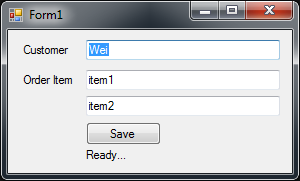
\includegraphics[scale=1.0]{Thread.PNG}
  \centering
  \caption{UI Thread Example\label{uithread}}
\end{figure}

This is a common problem that faces Windows developers. Suppose that when the Save button is clicked, a long running operation is triggered. Here we stimulate the long running operation by putting the thread to sleep. The label that says “Ready…” is updated to “OK” when the operation finishes.

\begin{lstlisting}[caption={Long running operation}, label=savedata1, frame=tb, basicstyle=\scriptsize]
public void SaveData ()
{
    //sleep to simulate long running process
    Thread.Sleep(10000);
    lblStatus.Text = "OK";
}
\end{lstlisting}

Window application is single thread application. While the long operation is in progress, the whole application will be unresponsive until the operation finishes. This makes a very bad user experience.

One remedy is to put the long running operation is a separate worker thread. And update the UI label when the worker thread finishes.

\begin{lstlisting}[caption={Long running operation with thread}, label=savedata2, frame=tb, basicstyle=\scriptsize]
public void SaveData ()
{
    new Thread(new ThreadStart(() =>
    {
        Thread.Sleep(5000);
        lblStatus.Text = "OK";
    })).Start();
}
\end{lstlisting}

But this would cause an exception to be thrown on line 6. UI elements can only be updated from the thread that created them.

\begin{lstlisting}[caption={Update UI from different thread}, label=savedata3, frame=tb, basicstyle=\scriptsize]
public void SaveData()
{ 
    Thread.Sleep(5000);
    Action action = () => lblStatus.Text = "OK";
    this.BeginInvoke(action);
}
\end{lstlisting}

Listing~\ref{savedata3} will marshal the request to update the UI back to the UI thread. Ensuring the label will be updated without any threading problem.
Since this is a common threading problem when working with UI. Buffalo can be used to extract the solution out as an aspect.

\begin{lstlisting}[caption={ThreadSafeAspect}, label=savedata4, frame=tb, basicstyle=\scriptsize]
public class ThreadSafeAspect : MethodAroundAspect
{
	public override object Invoke(Buffalo.MethodArgs args)
	{
		Dispatcher.CurrentDispatcher.Invoke(() => args.Proceed());
		return null;
	}
}
\end{lstlisting}

Here we create a new aspect inheriting from MethodAroundAspect, and overriding Invoke. This wraps around the invocation of the method call. Args.Proceed() is Buffalo’s way of calling back to the original UpdateStatus method.

\begin{lstlisting}[caption={Apply ThreadSafeAspect}, label=savedata5, frame=tb, basicstyle=\scriptsize]
public void SaveData()
{
	new Thread(new ThreadStart(() =>
	{
		Thread.Sleep(5000);
		this.UpdateStatus();
	})).Start();
}
[ThreadSafeAspect]
public void UpdateStatus() { lblStatus.Text = "OK"; }
\end{lstlisting}

Now when the Save button is clicked, the long running operation is triggered, control is immediately returned. When the operation finishes the label is updated without any threading issue.

Note that currently MethodAroundAspect supports only method level attribution. This limits its reusability. It will be much more useful when it support three levels as MethodBoundaryAspect does.


\section{Integrate With MS-Build System}

Buffalo can be integrated with MS-Build, so weaving can be invoked automatically when a project is compiled from the Visual Studio IDE. Note that the following instructions are just the bare minimum to get this working; a lot of bell and whistle are omitted.

MS-Build is integrated with Visual Studio IDE via configuration file. For example, a C\# project has the associated .csproj; if open in a text editor you will see a line that references a different configuration file: Microsoft.CSharp.targets. This file in term references Microsoft.Common.targets.

Each .NET version has its own Microsoft.Common.targets file. Depending on the version you are using, open up this file in a text editor. For example, for .NET 4.0, this file is located in C:\textbackslash Windows\textbackslash Microsoft.NET\textbackslash Framework\textbackslash v4.0.30319\textbackslash Microsoft.Common.targets.

Under the Compile section, around line \#2013, add the line to import the Buffalo.targets file as shown in figure~\ref{buffalo_targets}

\begin{figure}[H]
  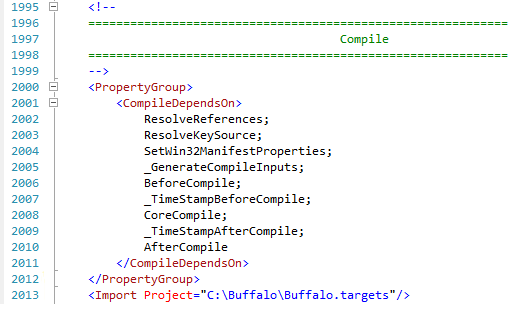
\includegraphics[scale=1.0]{CommonTarget.PNG}
  \centering
  \caption{Adding Buffalo.targets\label{buffalo_targets}}
\end{figure}

If you open Buffalo.targets in a text editor, it contains the following context:

\begin{lstlisting}[caption={Buffalo.targets}, label=buffalotargets, frame=tb, basicstyle=\scriptsize]
<Project xmlns="http://schemas.microsoft.com/developer/msbuild/2003">
  <PropertyGroup>
    <CompileDependsOn>
      $(CompileDependsOn);
      Buffalo
    </CompileDependsOn>
  </PropertyGroup>

  <Target Name="Buffalo">
    <Message Text="Hello Buffalo! @(IntermediateAssembly)"/>
    <Exec Command="&quot;C:\Buffalo\BuffaloAOP.exe&quot; &quot;@(IntermediateAssembly)&quot;"/>
  </Target>
</Project>
\end{lstlisting}

This is how Buffalo get hooked into MS-Build, what this mean is that when user compiles a project, everything defined in the CompileDependsOn property group will be performed first, then a new target named "Buffalo" will be called immediately, which will invoke the BuffaloAOP via the Exec Command. Note that for the Exec Command, a complete path to BuffaloAOP.exe must be provided, including the encoded quotation marks as shown.

Make sure to save all the changes. 

Now every time a C\# project is compiled, Buffalo will be invoked automatically to perform the weaving.
